\documentclass[11pt]{scrartcl}
\usepackage{graphicx}
\usepackage{ucs}
\usepackage[utf8x]{inputenc}
\usepackage[T1]{fontenc}
\usepackage[ngerman]{babel}
\usepackage[automark]{scrlayer-scrpage}
\usepackage{listings}
\usepackage{color}

\definecolor{eclipseBlue}{RGB}{42,0.0,255}
\definecolor{eclipseGreen}{RGB}{63,127,95}
\definecolor{eclipsePurple}{RGB}{127,0,85}

\lstset{
  basicstyle=\ttfamily\footnotesize,
  columns=fullflexible,
  showstringspaces=false,
  stepnumber=1,
  numbersep=5pt,
  backgroundcolor=\color{white},
  showspaces=false,
  showstringspaces=false,
  showtabs=false,
  frame=none,
  rulecolor=\color{black},
  tabsize=2,
  captionpos=b,
  breaklines=true,
  breakatwhitespace=false,
  title=\lstname,
  keywordstyle=\color{eclipseBlue},
  commentstyle=\color{eclipsePurple}\upshape
}
\lstdefinelanguage{XML}
{
  morestring=[s][\color{lightgreen}]{"}{"},
  morestring=[s][\color{black}]{>}{<},
  morecomment=[s]{<?}{?>},
  morecomment=[s][\color{green}]{<!--}{-->},
  stringstyle=\color{black},
  identifierstyle=\color{blue},
  morekeywords={xmlns,xsi,noNamespaceSchemaLocation,type,id,x,y,source,target,version,tool,transRef,roleRef,objective,eventually, dependencies, dependency}
}
\usepackage[colorlinks,
pdfpagelabels,
pdfstartview = FitH,
bookmarksopen = true,
bookmarksnumbered = true,
linkcolor = black,
plainpages = false,
hypertexnames = false,
citecolor = black] {hyperref}
\pagestyle{scrheadings}
\clearscrheadfoot
\ohead[]{\headmark}
\ofoot[]{\pagemark}

\title{Hochschule Düsseldorf - FB EI - Informatiklabor \newline Software-Engineering 2 Praktikum}
\author{Prof. Dr. Wolfgang Lux}
\date{\today{}, Düsseldorf}
\begin{document}
\maketitle
\tableofcontents

\newpage
\section{Einleitung}
\label{sec:introduction}

In diesem Praktikum soll ein REST-Server implementiert werden, 
der mit einem REST-Client angesprochen werden kann und die übertragenen Daten in einer
Datenbank abspeichert. Hierzu nutzen wir XAMPP, Java, Maven und Spring Boot.
Letzteres ist hier nur Mittel zum Zweck und soll nicht weiter vertieft werden.
Wir nutzen in diesem Praktikum die Java Entwicklungsumgebung Eclipse, es könnte - dank der Modularität von
Maven Projekten - auch jede andere Java Entwicklungsumgebung genutzt werden
wie Intellij IDEA, NetBeans, Visual Studio Code Java, etc \textit{(Genauso könnte auch Gradle anstelle 
von Maven genutzt werden um die externen Bibliotheken einzubinden)}.


\subsection{Wissenswertes}
\label{sec:wissenswertes}
\begin{itemize}
    \item \href{https://de.wikipedia.org/wiki/Eclipse_(IDE)}{Eclipse} oder 
    \href{https://code.visualstudio.com/docs/languages/java}{Visual Studio Code Java}
    \item \href{https://gluonhq.com/products/scene-builder/}{Gluon Scene Builder}
    \item \href{https://de.wikipedia.org/wiki/Annotation_(Java)}{Annotationen}
    \item \href{https://de.wikipedia.org/wiki/Generische_Programmierung_in_Java}{Generics}
    \item \href{https://de.wikipedia.org/wiki/Apache_Maven}{Maven}
    \item \href{https://spring.io/projects/spring-boot}{Spring Boot}
    \item \href{https://de.wikipedia.org/wiki/Hypertext_Transfer_Protocol}{HTTP} und \href{https://de.wikipedia.org/wiki/Representational_State_Transfer}{REST}
    \item \href{https://openjfx.io/}{JavaFX}
    \item \href{https://openjdk.java.net/projects/jigsaw/quick-start}{Java Module}
    \item \href{https://de.wikibooks.org/wiki/Muster:_Java:_Singleton}{Singletons}
\end{itemize}

\subsection{Idee}
\label{sec:idee}
JavaFX Client ---HTTP/JSON---> Spring Boot REST JPA Server ---> Datenbank \newline
JavaFX Client <---HTTP/JSON--- Spring Boot REST JPA Server <--- Datenbank

\subsection{Lernziele}
\label{sec:learninggoals}
\begin{itemize}
    \item Maven nutzen um externe Java Bibliotheken einzubinden
    \item Abstrakte Klassen, Abstrakte Methoden und Generics nutzen um Code-Duplikation zu vermeiden
    \item Spring Boot kennen lernen
    \item REST bzw. HTTP kennen lernen
    \item Java FX kennen lernen
\end{itemize}

\newpage
\section{Datenbank}
\label{sec:datenbank}

\subsection{XAMPP Installieren}
\label{sec:xamppinstallieren}
Um die Personendaten in einer MySQL oder MariaDB Datenbank abzuspeichern
empfiehlt es sich für Anfänger oder Testzwecke XAMPP zu nutzen, da die
grafische Oberfläche direkt mit
geliefert wird und es mit XAMPP einfach fällt den Zugriff auf eine Datenbank
einzurichten.\newline
XAMPP kann \textit{\textbf{entweder}} via Installer (Linux, MacOS, Windows) \textit{\textbf{oder}} via Docker Image
installiert werden.

\subsubsection{Installation via Installer}
\label{sec:installviainstaller}

\begin{enumerate}
    \item Dem Betriebssystem entsprechenden Installer von folgender Seite in \textit{Downloads}
          herunter laden: \url{https://www.apachefriends.org/de/download.html}
    \item Für Linux Nutzer: Installer ausführbar machen via Terminal (STRG + ALT + T)
          und anschließend ausführen via
          \begin{lstlisting}[language=bash]
        cd ~Downloads
        chmod +x xampp-linux-x64-7.4.7-0-installer.run
        sudo ./xampp-linux-x64-7.4.7-0-installer.run
    \end{lstlisting}
    \item Installations-Wizard durchklicken und XAMPP anschließend aufrufen.
\end{enumerate}

\newpage
\subsubsection{Oder: Install via Docker in Ubuntu Linux}
\label{sec:installviadocker}

\begin{enumerate}
    \item {Terminal aufrufen (STRG + ALT + T) und folgende Befehle nacheinander ausführen:
          \begin{lstlisting}[language=bash]
            sudo apt install docker.io
            sudo groupadd docker
            sudo usermod -aG docker $USER
            reboot
            docker pull cwsl/xampp
        \end{lstlisting}
          }
    \item \href{https://raw.githubusercontent.com/cswl/xampp-docker/master/xampp-docker.sh}{Script}
          aufrufen und in \textit{Downloads} abspeichern mit \textit{Seite speichern unter ...} (Firefox)
          oder \textit{Speichern unter ...} (Chrome)
    \item Terminal aufrufen (STRG + ALT + T) und folgende Befehle nacheinander
          ausführen, um das script ausführbar zu machen und es anschließend
          zu starten (was den XAMPP Container/Datenbank startet):
          \begin{lstlisting}[language=bash]
                cd ~/Downloads
                chmod +x xampp-docker.sh
                ./xampp-docker.sh
            \end{lstlisting}
    \item Falls keine IDE (Eclipse/VSCode) zum weiteren Betrieb genutzt wird, kann man
          den Container wieder mit dem Script stoppen:
          \begin{lstlisting}[language=bash]
        ./xampp-docker.sh stop
    \end{lstlisting}
\end{enumerate}

\newpage
\subsection{Benutzer und Datenbank erstellen}
\label{sec:benutzerstellen}

\begin{enumerate}
    \item \url{http://localhost:8086/phpmyadmin} aufrufen
    \item \textit{Benutzerkonten} anklicken
    \item \textit{Benutzerkonto hinzufügen} anklicken
    \item Benutzername ausdenken und einfügen
    \item Passwort ausdenken, einfügen und wiederholen
    \item WICHTIG: \textit{Erstelle eine Datenbank mit gleichen Namen und gewähre alle Rechte} anklicken!
    \item WICHTIG: \textit{Globale Rechte [ ] Alles auswählen} anklicken
    \item Alle anderen Einstellung unberührt lassen
    \item \textit{OK} anklicken
\end{enumerate}

\newpage
\section{Server}
\label{sec:server}

\subsection{Vorbereitung}
\label{sec:vorbereitung}

Eclipse unterscheidet zwischen dem Verzeichnis in dem es seinen Workspace
abspeichert und den Verzeichnissen in denen sich die Projekte befinden.
D.h. der Workspace kann in einem anderen Verzeichnis liegen als die Projekte
(Maven Projekte, Gradle Projekte, einfache Eclipse Java Projekte) -
alles kann aber auch in einem Verzeichnis liegen. In anderen IDEs
(Integrated Development Environment) muss der Workspace nicht undbedingt gewählt werden
 (Visual Studio Code). Wenn did Projekte erstellt sind, können sie aber in jeden 
 anderen Workspace importiert werden, wenn man das möchte.

\subsubsection{Workspace aussuchen}
\label{sec:workspaceaussuchen}

\begin{figure}[!ht]
    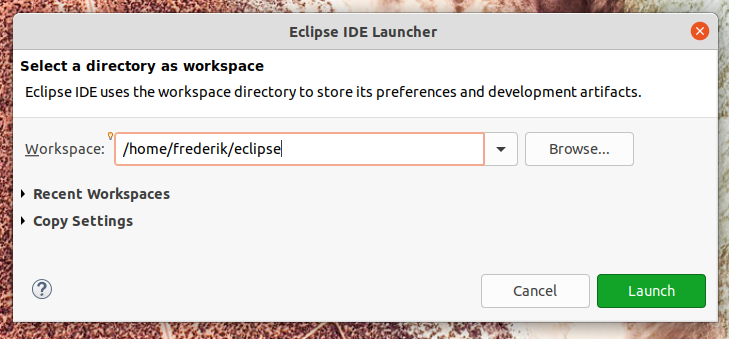
\includegraphics[width=\linewidth]{images/eclipse01_workspace.png}
    \caption{Workspace aussuchen}
    \label{fig:workspace}
\end{figure}

\newpage
\subsubsection{Maven Projekt erstellen}
\label{sec:mavenprojekterstellen}
\begin{figure}[!ht]
    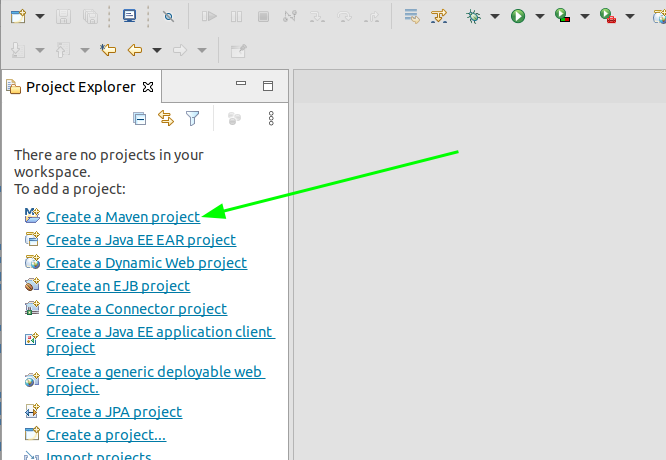
\includegraphics[width=\linewidth]{images/eclipse02_create_maven.png}
    \caption{Create a maven project}
    \label{fig:createmaven}
\end{figure}

\newpage
\begin{figure}[!ht]
    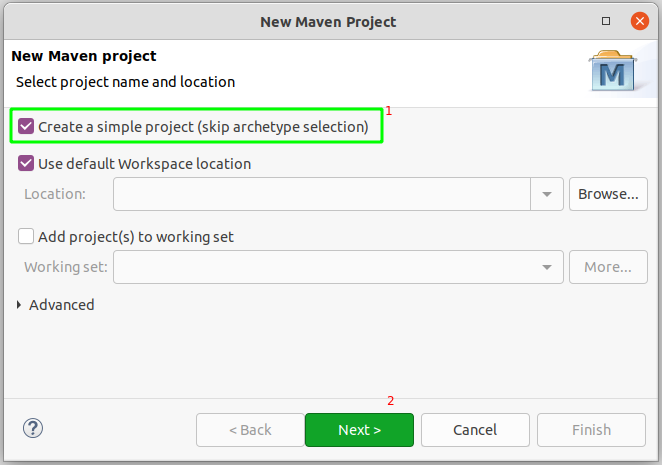
\includegraphics[width=\linewidth]{images/eclipse03_create_maven2.png}
    \caption{Skip archetype selection}
    \label{fig:createmaven2}
\end{figure}

\newpage
\begin{figure}[!ht]
    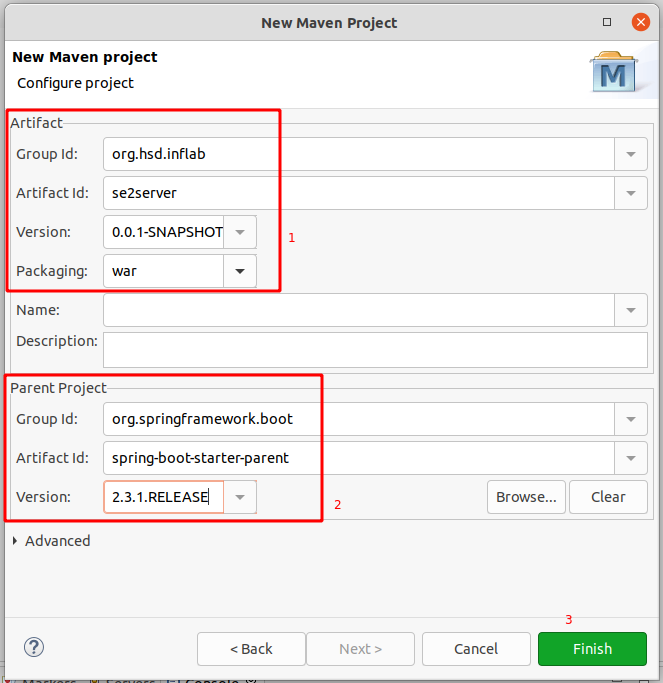
\includegraphics[width=\linewidth]{images/eclipse04_create_maven3.png}
    \caption{Fill the pom.xml file}
    \label{fig:createmaven3}
\end{figure}

\newpage
\subsubsection{Notwendige Java-Bibliotheken einbinden}
\begin{figure}[!ht]
    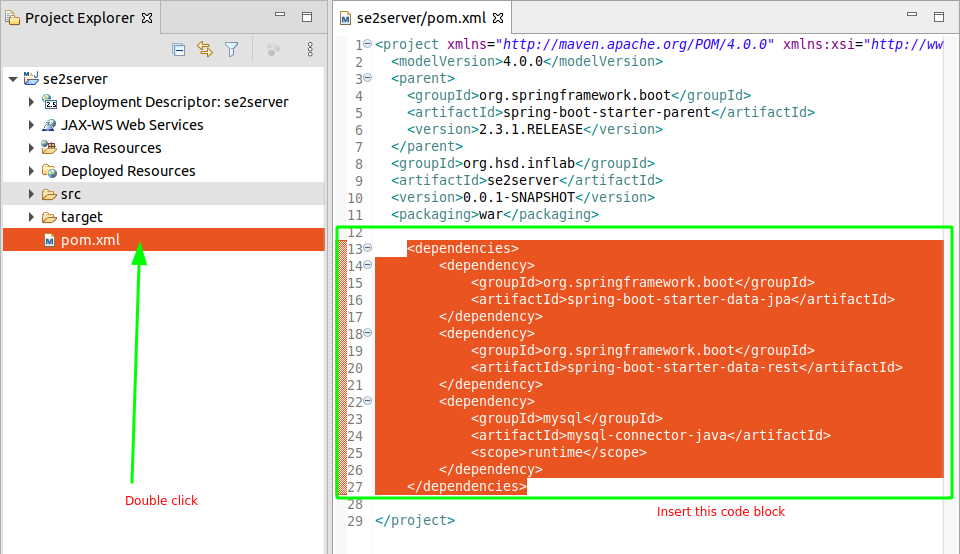
\includegraphics[width=\linewidth]{images/eclipse11_insert_dependencies.png}
    \caption{Abhängigkeiten einbinden}
    \label{fig:insertdependencies}
\end{figure}

\begin{enumerate}
    \item \textit{pom.xml} doppel-klicken
    \item folgenden Text unterhalb von \textit{<packaging>war</packaging>} und überhalb von
          \textit{</project>} einfügen:
          \begin{lstlisting}[language=XML]
    <dependencies>
        <dependency>
            <groupId>org.springframework.boot</groupId>
            <artifactId>spring-boot-starter-data-jpa</artifactId>
        </dependency>
        <dependency>
            <groupId>org.springframework.boot</groupId>
            <artifactId>spring-boot-starter-data-rest</artifactId>
        </dependency>
        <dependency>
            <groupId>mysql</groupId>
            <artifactId>mysql-connector-java</artifactId>
            <scope>runtime</scope>
        </dependency>
	</dependencies>
    \end{lstlisting}
\end{enumerate}

\newpage
\subsubsection{Applikation vorbereiten}
\label{sec:applicationprep}
Nun das Hauptpaket \textit{org.hsd.inflab.se2server} erstellen:
\begin{figure}[!ht]
    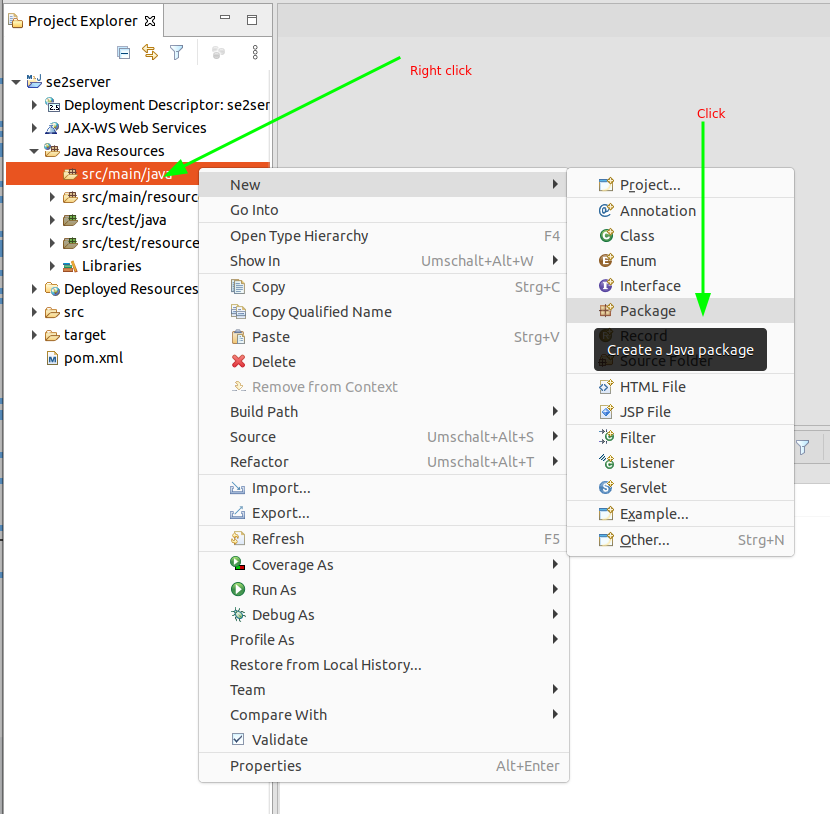
\includegraphics[width=\linewidth]{images/eclipse07_create_package.png}
    \caption{Create package}
    \label{fig:createpackage}
\end{figure}

\newpage
\begin{figure}[!ht]
    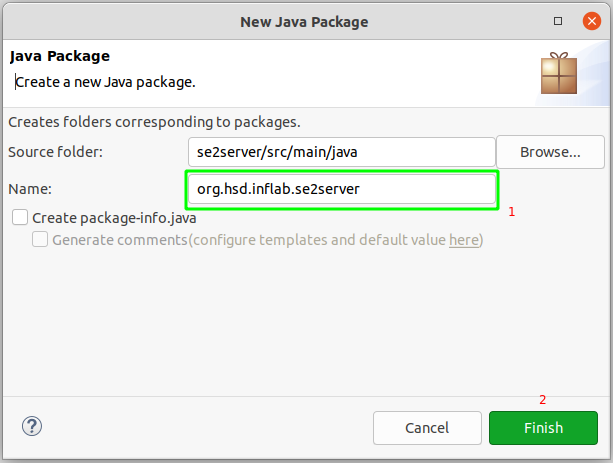
\includegraphics[width=\linewidth]{images/eclipse08_create_package2.png}
    \caption{Fill org.hsd.inflab.se2server into package name}
    \label{fig:createpackage2}
\end{figure}

\newpage
Innerhalb des Pakets die Klasse \textit{Application} erstellen:
\begin{figure}[!ht]
    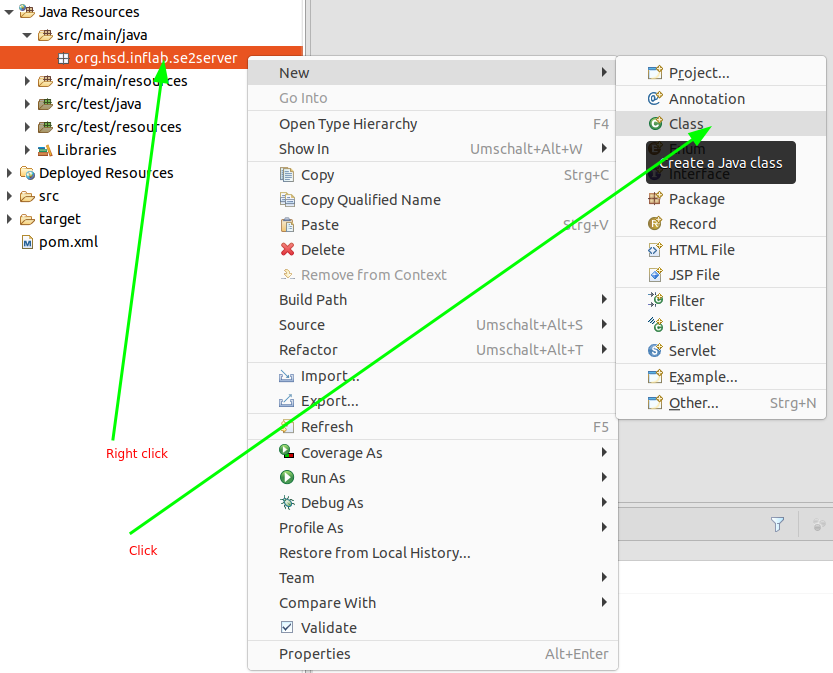
\includegraphics[width=\linewidth]{images/eclipse09_create_application_class.png}
    \caption{Create application class}
    \label{fig:createapplicationclass}
\end{figure}

\newpage
\begin{figure}[!ht]
    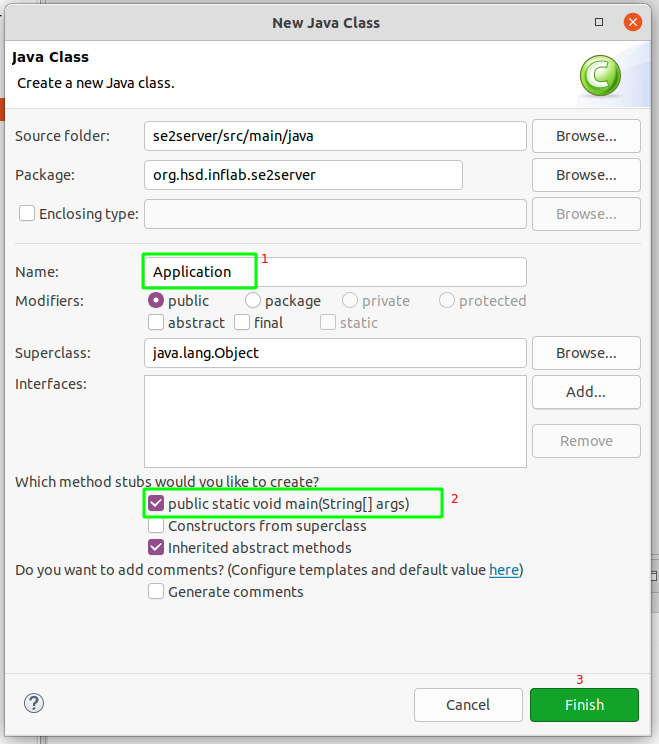
\includegraphics[width=\linewidth]{images/eclipse10_create_application_class2.png}
    \caption{Name it Application and click to insert main method}
    \label{fig:createapplicationclass2}
\end{figure}

\newpage
\subsubsection{Applikation startklar machen}
\label{customizeapplication}
Die gerade erstellte \textit{Application.java} öffnen und wie folgt anpassen:
\begin{enumerate}
    \item Über \textit{public class Application} folgende Annotation einfügen:
    \begin{lstlisting}[language=java]
    @SpringBootApplication
    \end{lstlisting}
    \item Innerhalb der \textit{main} Methode die Applikation wie folgt startbar machen:
    \begin{lstlisting}[language=java]
    SpringApplication.run(Application.class, args);
    \end{lstlisting}
    \item Fehlende imports nachladen (STRG + SHIFT + O)
    \item Speichern (STRG + S)
    \item in \textit{src/main/resources} die Datei \textit{application.properties}
          anlegen, und folgende properties dort einfügen
          (ADDRESS, DATABASENAME, USERNAME, PASSWORD anpassen... 
          wenn XAMPP mittels Installer installiert wurde, sollte ADDRESS \textit{localhost} sein
          wenn XAMPP in ein einem Docker Container läuft ist es dessen IP \textit{docker inspect -f '{{range .NetworkSettings.Networks}}{{.IPAddress}}{{end}}' xamppy-docker}):
    \begin{lstlisting}[language=java]
    spring.jpa.hibernate.ddl-auto=create-drop
    spring.datasource.url=jdbc:mysql://ADDRESS:3306/DATABASENAME
    spring.jpa.database-platform=org.hibernate.dialect.MySQL5Dialect
    spring.datasource.username=USERNAME
    spring.datasource.password=PASSWORD
    spring.jackson.serialization.fail-on-empty-beans=false
    spring.jpa.show-sql=true
    \end{lstlisting}
    \item \textit{Application.java} zu Testzwecken einmal starten
          (Rechtsklick -> Run as... -> Java application). Im späteren Verlauf natürlich neustarten,
          wenn Änderungen am Server vorgenommen werden.
\end{enumerate}

\newpage
\subsection{Server implementieren}
\label{sec:implementserver}
\subsubsection{Package Struktur erstellen}
\label{sec:createpackagestructure}
Innerhalb des Pakets \textit{org.hsd.inflab.se2server} mittels
\begin{figure}[!ht]
    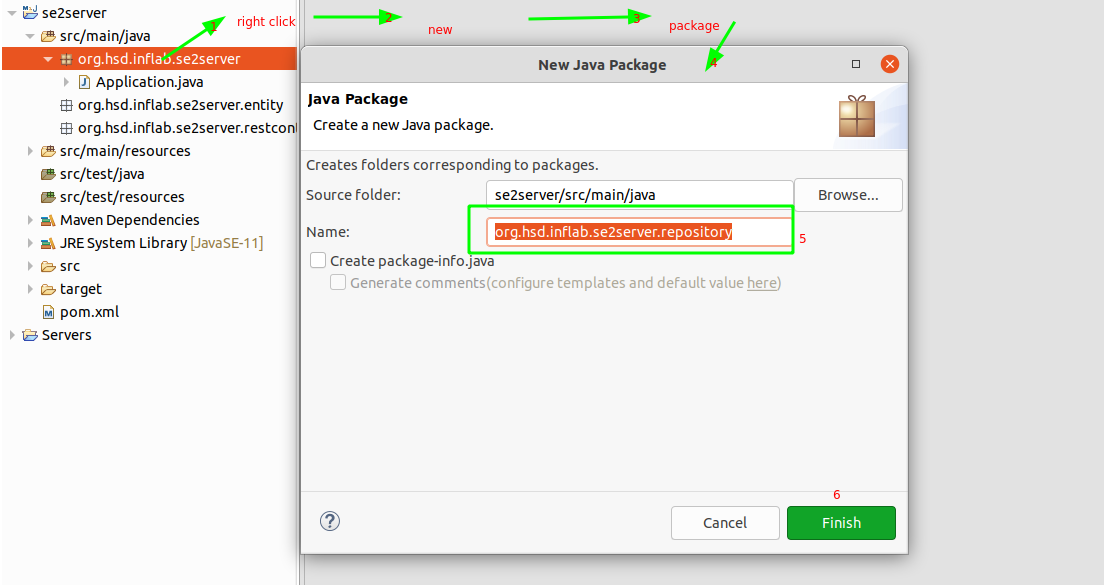
\includegraphics[width=\linewidth]{images/eclipse13_createpackages.png}
    \caption{Create packages}
    \label{fig:createpackages}
\end{figure}

folgende Pakete anlegen:
\begin{itemize}
    \item \textit{org.hsd.inflab.se2server.entity}
    \item \textit{org.hsd.inflab.se2server.repository}
    \item \textit{org.hsd.inflab.se2server.restcontroller}
\end{itemize}

\newpage
\subsubsection{AbstractEntity und Person erstellen}
\label{sec:createentities}
Innerhalb des \textit{entity} Pakets die Klassen \textit{AbstractEntity}, die abstrakte Klasse 
die das Id Feld enthält und die konkrete Entity 
und \textit{Person} anlegen, welche von AbstractEntity erbt:
\begin{lstlisting}[language=java]
package org.hsd.inflab.se2server.entity;

import java.io.Serializable;

import javax.persistence.Column;
import javax.persistence.GeneratedValue;
import javax.persistence.Id;
import javax.persistence.MappedSuperclass;

import com.fasterxml.jackson.annotation.JsonIgnoreType;

@SuppressWarnings("serial")
@MappedSuperclass
public abstract class AbstractEntity implements Serializable {

    @Id
    @GeneratedValue
    @Column(unique = true)
    long id;

    public long getId() {
        return id;
    }

    public void setId(long id) {
        this.id = id;
    }
    
}
\end{lstlisting}

\newpage
\begin{lstlisting}[language=java]
package org.hsd.inflab.se2server.entity;

import javax.persistence.Entity;

@Entity
public class Person extends AbstractEntity {
    
    private static final long serialVersionUID = -3421268250084118586L;
    private String name;

    public String getName() {
        return name;
    }

    public void setName(String name) {
        this.name = name;
    }

    public Person() {
    }
    
}
\end{lstlisting}

\subsubsection{Repositories erstellen}
\label{sec:createrepository}

Innerhalb des Pakets \textit{repository} die zwei Interfaces \textit{GenericRepository.java} und 
\textit{PersonRepository.java} anlegen. Diese Interfaces werden von Spring Boot dazu genutzt um mit der Datenbank
zu kommunizieren. Sie nehmen den Platz ein, den in händisch programmierten ORMs ein DAO einnehmen würde.
Angenehmer Weise müssen wir nichts weiteres tun, als diese leeren Inerfaces zu erstellen.
Eigentlich bräuchten wir nur ein Repository (PersonRepository), da wir aber einen GenericRestService 
eines bestimmten Typs von AbstractEntity nutzen wollen, müssen wir auich das Repository generisch halten.
\begin{lstlisting}[language=java]
package org.hsd.inflab.se2server.repository;
import ... // STRG + SHIFT + O
public abstract interface GenericRepository<T extends AbstractEntity> extends JpaRepository<T, Serializable> { }
\end{lstlisting}

\begin{lstlisting}[language=java]
package org.hsd.inflab.se2server.repository;
import org.hsd.inflab.se2server.entity.Person;
public interface PersonRepository extends GenericRepository<Person> { }    
\end{lstlisting}


\newpage
\subsubsection{GenericRestController und PersonRestController erstellen}
\label{sec:createcontroller}

Innerhalb des Paktes \textit{restcontroller} die Klassen 
\textit{GenericRestController.java} und \textit{PersonRestController.java}
erstellen. Diese RestController ermöglichen die REST Schnittstelle
und machen unseren REST-Server erst zu solchem. Die Methoden list(), read(),
update() und delete() sind nach dem CRUD prinzip erstellt und 
entsprechend genau den Methoden des HTTP Protokolls (GET, POST, PUT, DELETE).
Dies wird mittels entsprechender Annotationen (@GetMapping, etc) gekennzeichnet
und Spring ruft diese Methoden dann auf, wenn die Adresse des Servers 
mittels Http GET, POST, PUT und DELETE angesprochen wird.
Innherhalb der Methoden wird unser GenericRepository angesprochen,
welches die entsprechenden MySQL Befehle absetzt um entweder 
Tabellenspalten auszulesen, zu ändern, zu erstellen oder zu löschen.
Was wir nicht generisch gestalten können, ist auf welche Weise
ein Tabelleneintrag aktualisiert wird, da wir nicht wissen, welche 
Spalten unsere Tabelle enthält bzw. welche Felder unsere Entity hat.
Daher ist die Methode \textit{updateEntity(E e, E newE)} abstrakt.
Die Implementierung ist das Einzige was die konkrete Klasse 
PersonRestController nachliefern muss.
Ebenfalls sind die Annotationen \textit{@RestController} was Spring sagt
das hier unser RestController zu finden ist und \textit{@RequestMapping("/persons")}
was den Namen der Resource Person definiert, nur für die konkrete Klasse 
angegeben.

\newpage
\begin{lstlisting}[language=java]
package org.hsd.inflab.se2server.restcontroller;
import ... // imports nachladen mit (STRG + SHIFT + O)

public abstract class GenericRestController<E extends AbstractEntity> {
    
    protected abstract E updateEntity(E e, E newE);
    
    @Autowired
    protected GenericRepository<E> repository;

	@GetMapping
	public List<E> list() {
		return repository.findAll();
	}	
	@PostMapping
	public E create(@RequestBody E entity) {
		return repository.save(entity);
	}	
	@DeleteMapping("{id}")
	public void delete(@PathVariable(value = "id") long id) {
		repository.deleteById(id);
	}	
	@GetMapping("{id}")
	public E get(@PathVariable(value = "id") long id) {
		return repository.getOne(id);
	}
    @PutMapping("{id}")
    public E update(@PathVariable long id, @RequestBody E newE) {

        return repository.findById(id).map(e -> {
            e = updateEntity(e, newE);

			return repository.save(e);

        }).orElseGet(() -> {
            newE.setId(id);
            return repository.save(newE);
        });        
    }
}
\end{lstlisting}
\newpage
\begin{lstlisting}[language=java]
package org.hsd.inflab.se2server.restcontroller;

import org.hsd.inflab.se2server.entity.Person;
import org.springframework.web.bind.annotation.RequestMapping;
import org.springframework.web.bind.annotation.RestController;

@RestController
@RequestMapping("/persons")
public class PersonRestController extends GenericRestController<Person> {

    @Override
    protected Person updateEntity(Person e, Person newE) {
        e.setName(newE.getName());

        return e;
    }    
    
}
\end{lstlisting}

\subsubsection{Server testen}
\label{sec:servertest}

Die REST Schnittstelle um eine Person(en) erstellen, löschen, editieren und als Liste
ausgeben zu lassen ist nun implementiert.\newline
Dies können wir auf unterschiedliche Weise bzw. mit unterschiedlichen REST Clients (Programmen)
testen. Für Chome gibt es die Extension \textit{Advanced REST client} für Firefox
gibt es die Extension \textit{RESTED}. Für Linux und Windows kann auch über ein Terminal
das Kommandozeilenprogramm \textit{curl} genutzt werden. Für Visual Studio Code gibt es
ebenfalls diverse REST extensions. Es ist vollkommen egal was genutzt wird, die Hauptsache
ist dass HTTP Befehle an den Server geschickt werden. Dieser Antwortet mit HTTP
genau wie sie das von ihrem Browser und Websites kennen. Dort fragen sie mit HTTP GET 
eine bestimme Adresse ab (http://www.google.de) und der Webserver der sich hinter der Adresse
verbirgt antwortet mit HTTP und einer HTML Datei im Body welche wiederum ihr Browser
versteht und mit einer HTML Render Engine (Chrome: Blink, Firefox: Gecko/Quantum) umwandelt
in eine Website so wie Sie das nun eben aus dem Internet gewohnt sind.

\newpage
\section{Client}
\label{sec:client}

\subsection{Vorbereitung}
\label{sec:clientsetup}

\subsubsection{Maven Projekt nach Archetyp erstellen}
\label{sec:clientmaven}

Diesmal das Mavenprojekt nach einem Archetyp erstellen. 
Dies spart in der Regel Zeit, wenn man vorher weiß
welche externen (im Sinne von "nicht in der JDK mitgeliefert")
Java-Bibliotheken man einbinden möchte. Rechtsklick auf eine
freie Stelle im Package Explorer und mit 
\textit{New --> Other... --> Suche nach Maven --> Maven Project}
ein neues Maven Projekt erstellen.
\begin{figure}[!ht]
    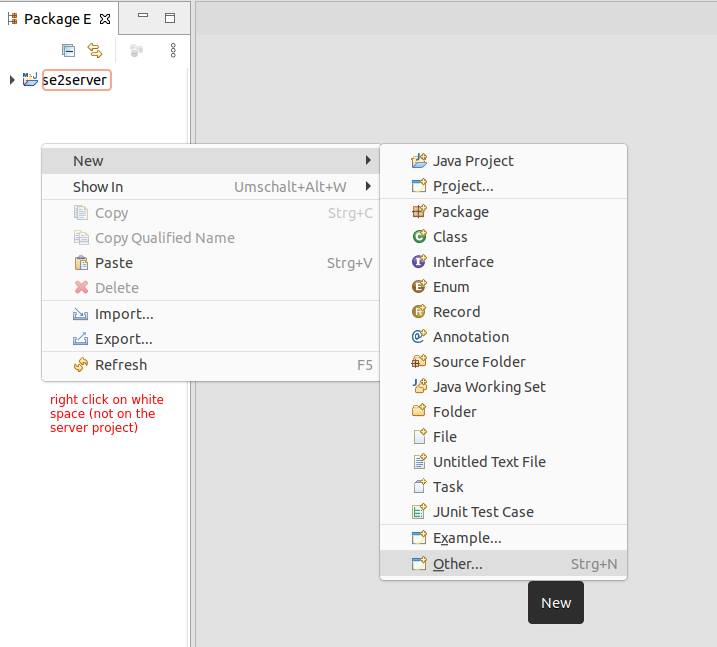
\includegraphics[width=\linewidth]{images/eclipse14_client_maven_project.png}
    \caption{Create client maven project}
    \label{fig:createclientproject}
\end{figure}

\newpage
\begin{figure}[!ht]
    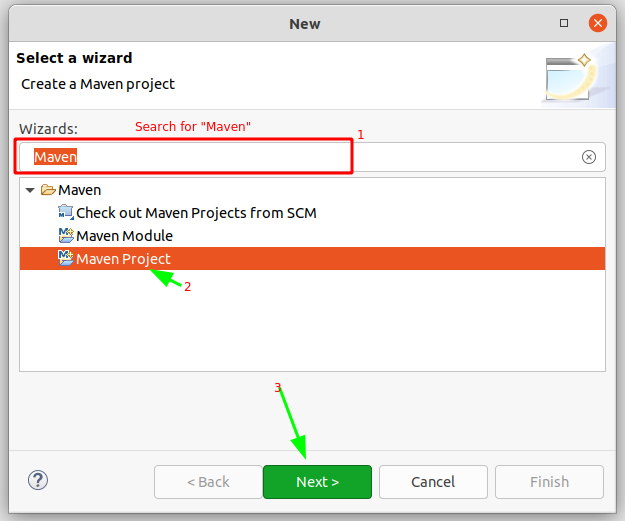
\includegraphics[width=\linewidth]{images/eclipse15_client_maven_project2.png}
    \caption{Create client maven project2}
    \label{fig:createclientproject2}
\end{figure}

\newpage
Diesmal unbedingt \textit{Create a simple project (skip archetype selection)}
NICHT anklicken und mit \textit{Next>} zum nächsten Wizard-Schritt wechseln
\begin{figure}[!ht]
    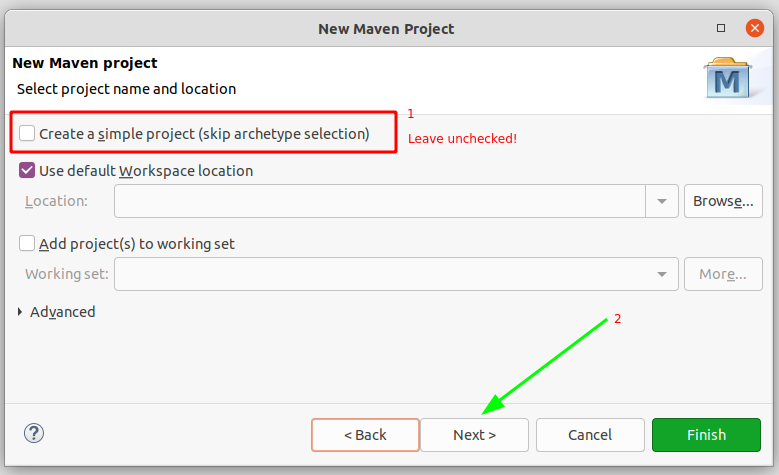
\includegraphics[width=\linewidth]{images/eclipse16_client_maven_project3.png}
    \caption{Create client maven project3}
    \label{fig:createclientproject3}
\end{figure}

\newpage
Im Filter Textfeld nach \textit{javafx} suchen und die Zeile
\textit{org.openjfx javafx-archetype-fxml} aussuchen:
\begin{figure}[!ht]
    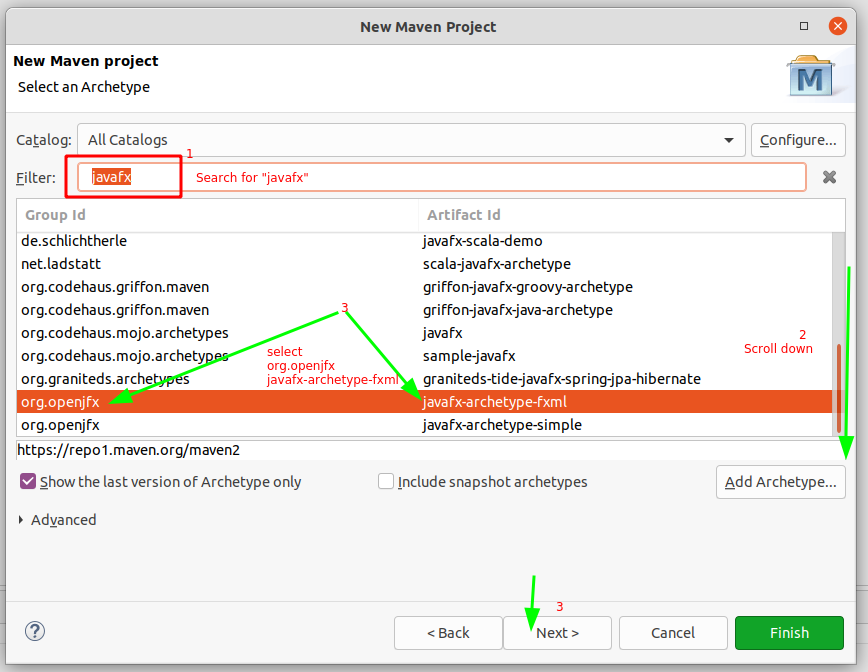
\includegraphics[width=\linewidth]{images/eclipse17_client_maven_project4.png}
    \caption{Create client maven project4}
    \label{fig:createclientproject4}
\end{figure}

\newpage
Nun wieder die Group id \textit{org.hsd.inflab} aber die artifactId
\textit{se2fxclient} eingeben. Das Package soll unbedingt \textit{org.hsd.inflab.se2fxclient}
heißen: \newline
\begin{figure}[!ht]
    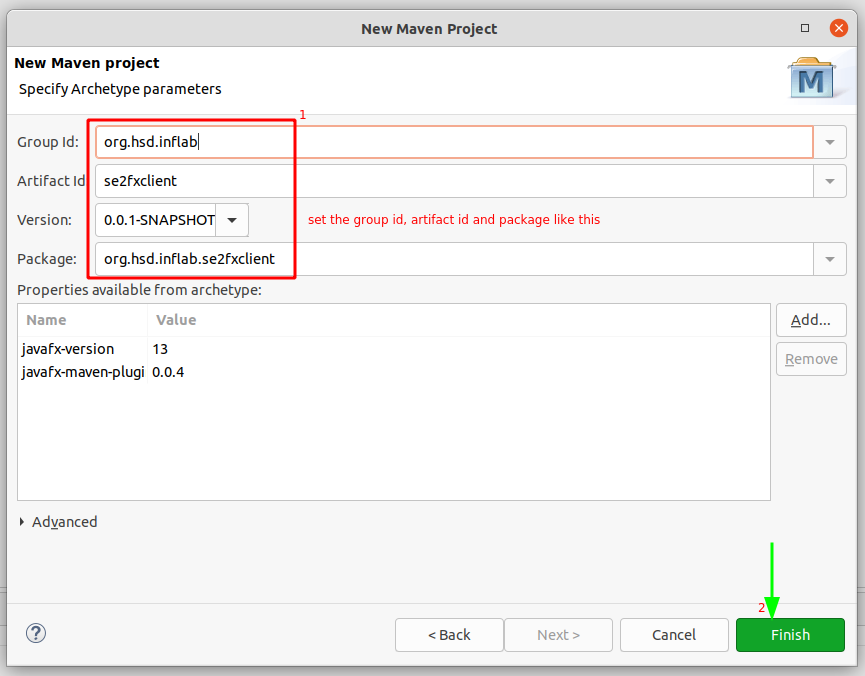
\includegraphics[width=\linewidth]{images/eclipse18_client_maven_project5.png}
    \caption{Create client maven project5}
    \label{fig:createclientproject5}
\end{figure}

\textbf{WICHTIG}: Es wurde nun bereits eine pom.xml, eine Standart Application Klasse,
ein Controller und zwei fxml Dateien angelegt. App.java, Controller.java
und die zwei fxml Dateien sollen nun gelöscht werden. Da wir nur die pom.xml benötigen (und die Struktur).
Alles Weitere wird in den nächsten Schritten händisch angelegt.

\newpage
\subsubsection{pom.xml anpassen}
\label{customizepom}
Für die REST-Schnittstelle zum Server bzw. für Zugriff auf HTTP benötigen wir
noch eine Bibliothek um einen HttpClient zu nutzen. Um JSON zu verarbeiten eine weitere.
Daher muss die \textit{pom.xml} des Clients um folgende zwei \textit{dependencies} erweitert
werden:

\begin{lstlisting}[language=XML]
<dependency>
    <groupId>org.apache.httpcomponents</groupId>
    <artifactId>httpclient</artifactId>
    <version>4.5.9</version>
</dependency>
<dependency>
    <groupId>org.json</groupId>
    <artifactId>json</artifactId>
    <version>20190722</version>
</dependency>
\end{lstlisting}

\textbf{ACHTUNG}: Wir nutzen den HttpClient von Apache und nicht den inkludierten
HttpClient des JDK, da wir uns bei letzterem selber 
darum kümmern müssten, die geöffneten Verbindungen in der richtigen Reihenfolge
wieder zu schließen. Wenn die Importe also mit STRG + SHIFT + O im Folgenden
nachgeladen werden, ist es wichtig die Klassen aus
\textit{org.apache.http.*} zu importieren!

\newpage
\subsection{Client implementieren}
\label{sec:implementclient}
\subsubsection{Paketstruktur erstellen}
\label{sec:createpaketstructure}

Nacheinader in \textit{src/main/java} folgende Pakete ...
\begin{itemize}
    \item \textit{org.hsd.inflab.se2fxclient.model}
    \item \textit{org.hsd.inflab.se2fxclient.view}
    \item \textit{org.hsd.inflab.se2fxclient.controller}
    \item \textit{org.hsd.inflab.se2fxclient.service}
\end{itemize}
\begin{figure}[!ht]
    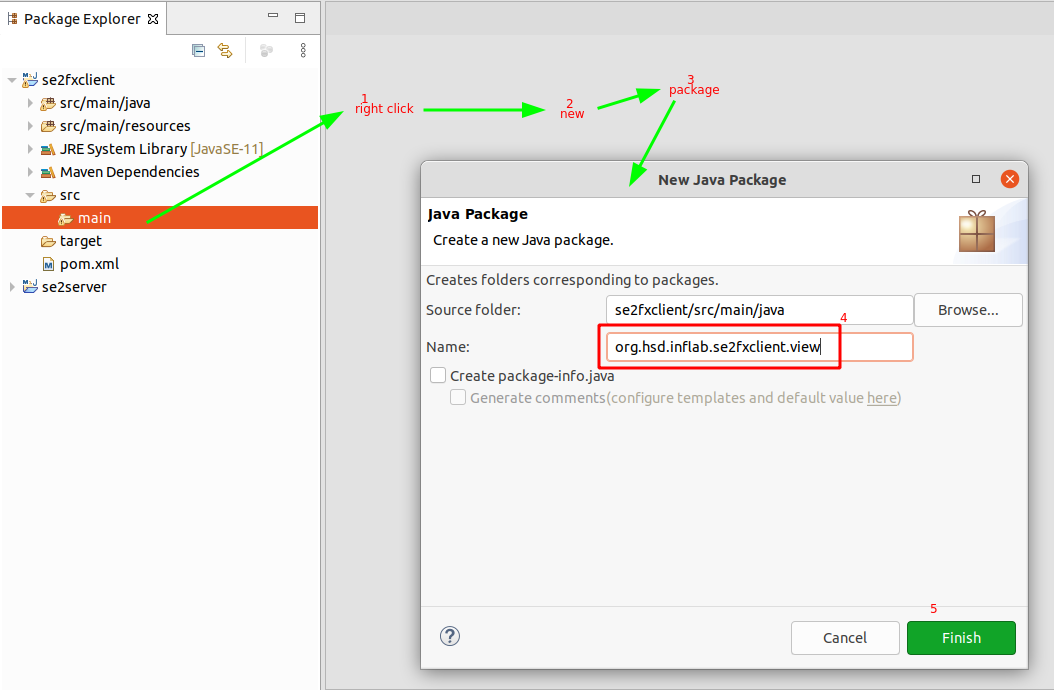
\includegraphics[width=\linewidth]{images/eclipse19_client_package.png}
    \caption{Create client packages}
    \label{fig:createclientpackages}
\end{figure}

\newpage
...und in \textit{src/main/resources} die \textit{FOLDER} mit 
Namen \textit{view} und \textit{service} anlegen.

\begin{figure}[!ht]
    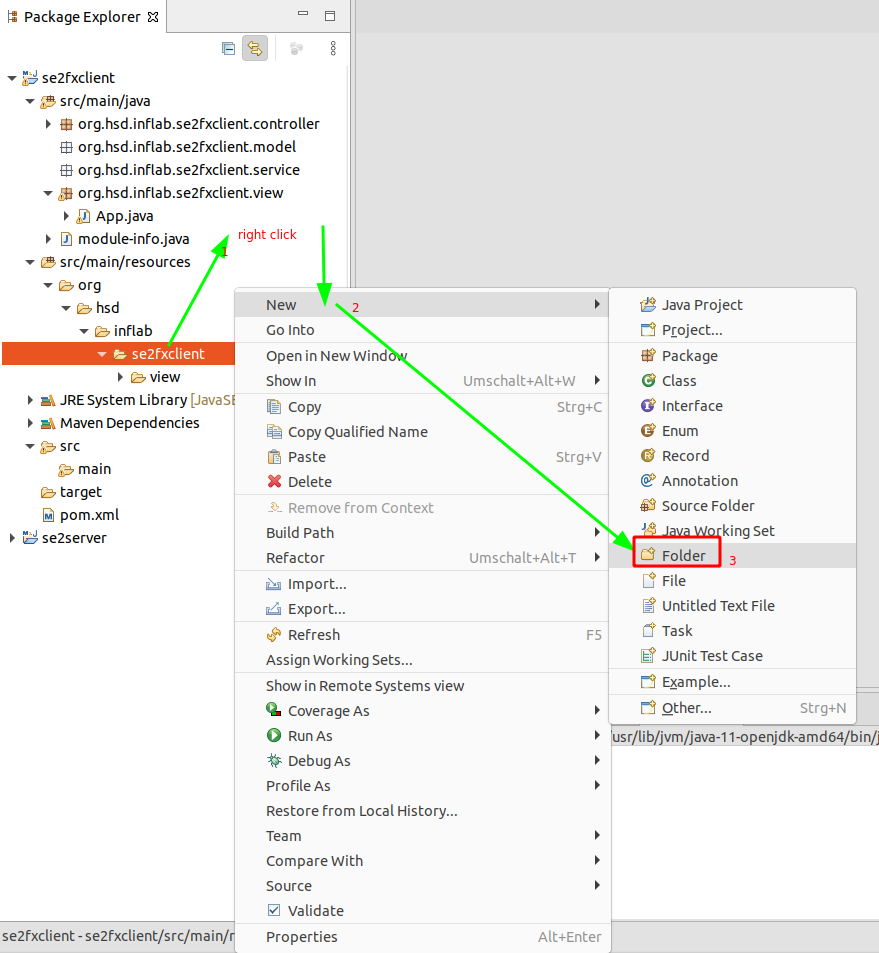
\includegraphics[width=\linewidth]{images/eclipse22_client_resource_folder2.png}
    \caption{Create client resource folder2}
    \label{fig:createclientresourcefolder2}
\end{figure}

\newpage
\begin{figure}[!ht]
    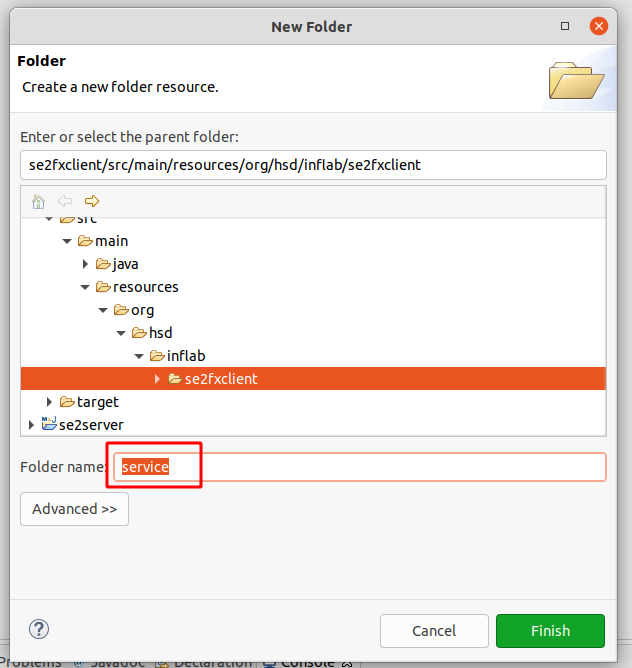
\includegraphics[width=\linewidth]{images/eclipse22_client_resource_folder3.png}
    \caption{Create client resource folder3}
    \label{fig:createclientresourcefolder3}
\end{figure}

\newpage
\begin{figure}[!ht]
    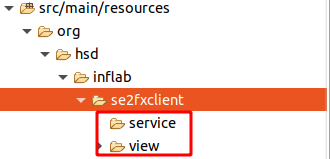
\includegraphics[width=\linewidth]{images/eclipse22_client_resource_folder.png}
    \caption{Create client resource folder}
    \label{fig:createclientresourcefolder}
\end{figure}

\newpage
\subsubsection{Module Info konfigurieren}
\label{sec:moduleinfo}
\textbf{WICHTIG}: Seit Java9 ist es zwingend notwendig die JavaFX Module einzubinden.
Dies geschieht in der Datei \textit{module-info.java} - zunächst Zeile
6 und  7 auskommentieren, da das \textit{controller} Paket momentan leer ist.
\begin{figure}[!ht]
    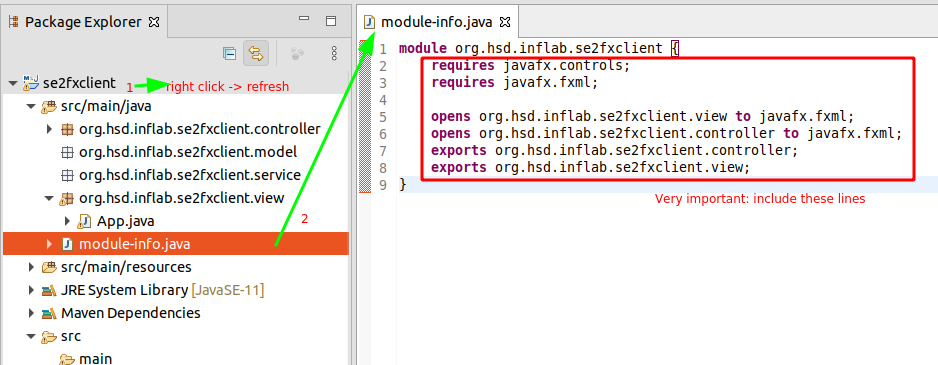
\includegraphics[width=\linewidth]{images/eclipse21_client_module_info.png}
    \caption{Edit module info}
    \label{fig:editmoduleinfo}
\end{figure}

\newpage
\subsubsection{Die App-Klasse anlegen}
\label{sec:createappclass}
Im java Paket \textit{view} die Klasse \textit{App} anlegen,\newline
das Häkchen bei \textit{public static void main(String[] args)} setzen
und als \textit{Superclass} die Klasse \textit{Application} aus dem
Paket \textit{javafx.application} setzen.

\begin{figure}[!ht]
    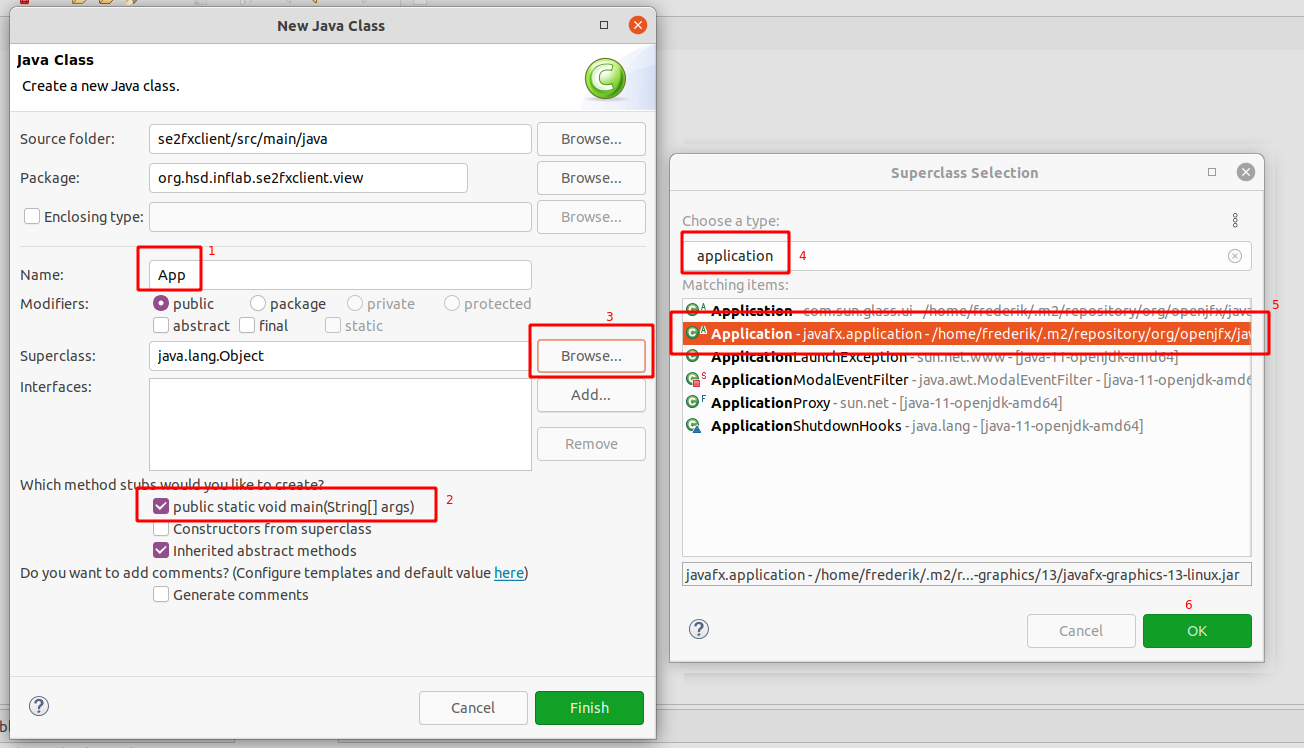
\includegraphics[width=\linewidth]{images/eclipse20_client_app.png}
    \caption{Create client app}
    \label{fig:createclientapp}
\end{figure}

\newpage
\subsubsection{App-Klasse befüllen}
\label{sec:fillappclass}

Die Klasse \textit{App} mit folgendem Code befüllen (die Importe nachladen):

\begin{lstlisting}[language=java]
package org.hsd.inflab.se2fxclient.view;

import java.io.IOException;

import ... // STRG + SHIFT + O

public class App extends Application {

    @Override
    public void start(Stage stage) throws IOException {
        FXMLLoader fxmlLoader = new FXMLLoader(App.class.getResource("PersonView.fxml"));
        Scene scene = new Scene(fxmlLoader.load());
        stage.setScene(scene);
        stage.show();
    }

    public static void main(String[] args) {
        launch();
    }
}    
\end{lstlisting}

\newpage
\subsubsection{FXML Datei anlegen}
\label{sec:createfxml}

SceneBuilder öffnen und eine neue Datei anlegen,
links aus dem Bereich \textit{Containers} den Container
\textit{BorderPane} in die Arbeitsfläche ziehen\newline und die Datei als \textit{PersonView.fxml}
in ihrem System im Projekt
in \textit{se2fxclient/src/main/resources/org/hsd/inflab/se2fxclient/view} abspeichern:

\begin{figure}[!ht]
    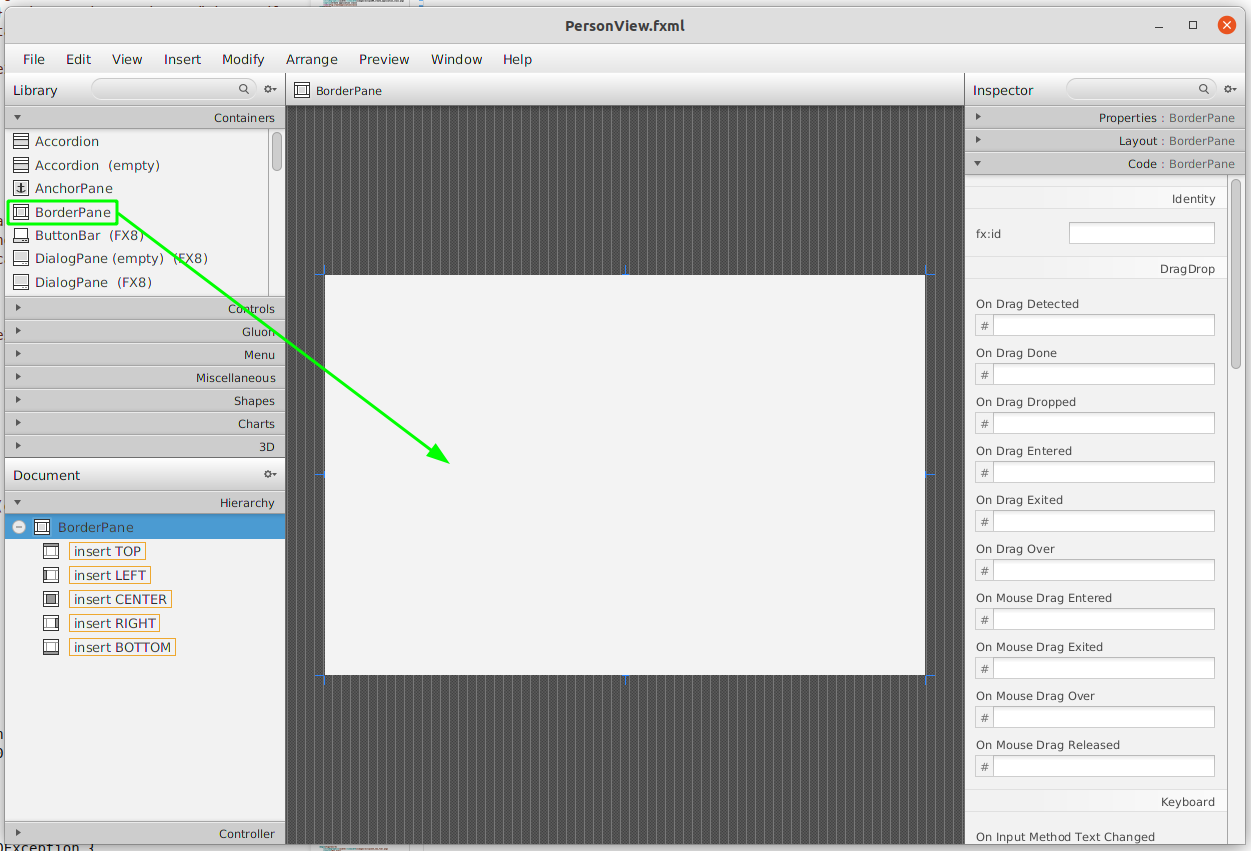
\includegraphics[width=\linewidth]{images/eclipse23_new_fxml.png}
    \caption{New fxml}
    \label{fig:newfxml}
\end{figure}

\newpage
\subsubsection{App testen}
\label{sec:apptest}
In Eclipse rechtsklick auf \textit{App.java} und mit \textit{Run as-->Java Application}
die Applikation starten...
\begin{figure}[!ht]
    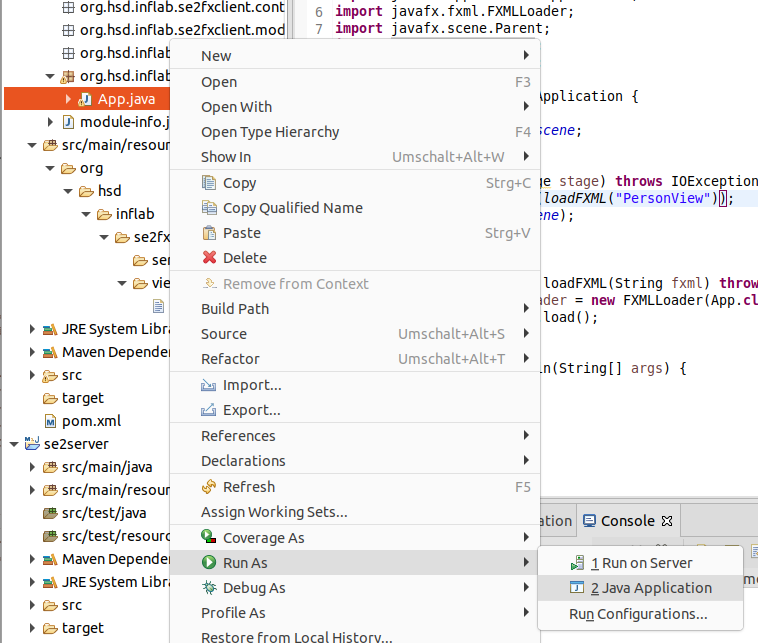
\includegraphics[width=\linewidth]{images/eclipse24_test_app.png}
    \caption{Test App}
    \label{fig:testapp}
\end{figure} und ein Fenster mit weißem Hintergrund erscheint (hoffentlich):
\newpage
\begin{figure}[!ht]
    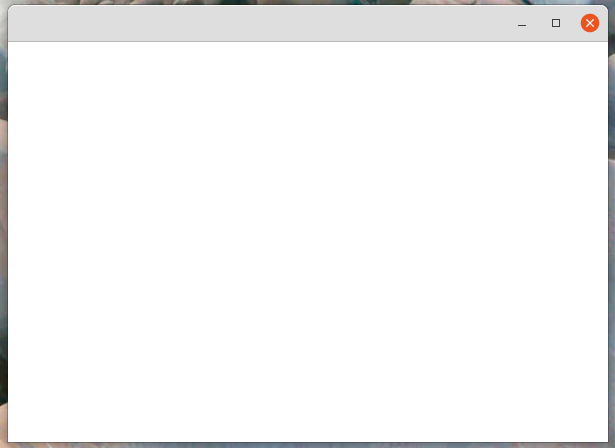
\includegraphics[width=\linewidth]{images/eclipse25_test_app2.png}
    \caption{Test App2}
    \label{fig:testapp2}
\end{figure}

\newpage
\subsubsection{Model Klassen}
\label{sec:modelclasses}
Jede Person soll auf allen Schichten abgebildet werden. Zunächst
als einfache ModelKlasse \textit{Person.java} welche von \textit{AbstractModel.java}
das Attribut \textit{id} erbt:
\begin{lstlisting}[language=java]
package org.hsd.inflab.se2fxclient.model;

public class AbstractModel {
    
    int id;

    public int getId() {
        return id;
    }

    public void setId(int id) {
        this.id = id;
    }
}    
\end{lstlisting}

\begin{lstlisting}[language=java]
package org.hsd.inflab.se2fxclient.model;

public class Person extends AbstractModel {

    String name;

    public String getName() {
        return name;
    }

    public void setName(String name) {
        this.name = name;
    }

    public Person() {
    }

    public Person(String name) {
        this.name = name;
    }    
}
\end{lstlisting}

\newpage
\subsubsection{Service Klassen erstellen}
\label{sec:serviceclasses}

Der Server gibt vor wie mit der Datenbank gesprochen wird, nämlich
nach dem CRUD-Prinzip: create(), read()/readAll() bzw. list(), update(), 
delete(). Genauso werden auch 
die Methoden des Service benannt. Innerhalb der Methoden wird
ein HttpClient erstellt und am Ende der Methode mittels finalize 
auf jeden Fall auch wieder geschlossen (das Schließen ist nötig, da ansonsten
immer mehr offene Ports erstellt und nie wieder geschlossen würden,
was letztendlich zum Absturz des Programms führen könnte).
Mit Hilfe der Json Bibliothek, werden entweder aus vorhanden ModelObjekten 
JsonObjekte gebaut, oder aus empfangenen JsonObjekten
ModelObjekte. Die create() Methode versendet mit Hilfe des HTTP POST 
Befehls ein Model in Form eines JsonObjekts, allerdings ohne Id, da diese
nur von der Datenbank vergeben wird. Die HttpResponse 
enthält das Vollständige JsonObjekt inklusive der Id.
Das JsonObjekt wird anschließend wieder in ein ModelObjekt 
umgewandelt und von der Methode als Rückgabewert zurück gegeben.
Entsprechend sendet delete(...) ein HTTP DELETE, readAll() ein HTTP GET und
update(...) ein HTTP PUT.


\textit{Model} steht in dem Fall für eine einfache Java Klasse (also keine grafischen
Klassen nutzt, oder andere komplizierte Logik beinhaltet).
Da wir nicht für jedes mögliche ModelObjekt den ganzen Service Code 
neu schreiben wollen, erstellen wir den Service als 
generische, abstrakte Klasse. Dieser enthält alle wichtigen Methoden
um mit dem Server zu kommunizieren. 
Das Einzige was wir nicht vorhersagen können, ist welche 
Felder eine zukünftige ModelKlasse haben könnte. Daher 
erstellen wir die abstrakten, das heißt ohne Implementierung, Methoden
\textit{createJSONObjectFromModelObject(M m)} und \textit{createModelObjectFromJSONObject(JSONObject jsonObject)}.
Wenn ein RestService von GenericRestService erben möchte, wird
er dadurch gezwungen die Methoden zu implementieren.
Denn nur innerhalb dieses konkreten Service ist klar, welche
Felder die neue ModelKlasse beinhaltet.


\begin{lstlisting}[language=java]
package org.hsd.inflab.se2fxclient.service;

import ... // STRG + SHIFT + O

public abstract class GenericRestService<M extends AbstractModel> {
    
    private static String baseUrl;
    private static String url;
    protected abstract String getResourceName();
    protected abstract JSONObject createJSONObjectFromModelObject(M m);
    protected abstract M createModelObjectFromJSONObject(JSONObject jsonObject);
    
    protected void createURL() {
        loadProperties();
        url = new String(baseUrl + "/" + getResourceName());
    }

    public GenericRestService() {
        createURL();
    }

    public boolean connectionIsWorking() {
        try (CloseableHttpClient client = HttpClientBuilder.create().build()) {
            HttpGet request = new HttpGet(baseUrl);
            HttpResponse response = client.execute(request);
            return response.getStatusLine().getStatusCode() == HttpStatus.SC_OK;
        } catch (IOException e) {
            e.printStackTrace();
            return false;
        }        
    }

    public static void loadProperties() {
        Properties properties = new Properties();
        try {
            properties.load(GenericRestService.class.getResourceAsStream("connections.properties"));
        } catch (IOException e) {
            e.printStackTrace();
        }
        baseUrl = properties.getProperty("base.url");
    }

    public M create(M m) {
        JSONObject jsonObject = createJSONObjectFromModelObject(m);
        HttpPost request = new HttpPost(url);
        HttpResponse response;
        request.setHeader(HttpHeaders.CONTENT_TYPE, "application/json");

        try (CloseableHttpClient client = HttpClientBuilder.create().build()) {
            request.setEntity(new StringEntity(jsonObject.toString()));
            response = client.execute(request);
            BufferedReader bufferedReader = new BufferedReader(
                    new InputStreamReader(response.getEntity().getContent()));
            StringBuilder stringBuilder = new StringBuilder();
            String line = "";
            while ((line = bufferedReader.readLine()) != null) {
                stringBuilder.append(line);
                System.out.println(line);
            }
            JSONObject personJSON = new JSONObject(stringBuilder.toString());
            m.setId(personJSON.getInt("id"));
        } catch (IOException e) {
            e.printStackTrace();
        }
        return m;
    }

    public List<M> readAll() {
        HttpGet request = new HttpGet(url);
        HttpResponse response;
        List<M> list = new ArrayList<>();
        try (CloseableHttpClient client = HttpClientBuilder.create().build()) {
            response = client.execute(request);
            BufferedReader bufferedReader = new BufferedReader(
                    new InputStreamReader(response.getEntity().getContent()));
            StringBuilder stringBuilder = new StringBuilder();
            String line = "";
            while ((line = bufferedReader.readLine()) != null) {
                stringBuilder.append(line);
            }
            JSONArray jsonArray = new JSONArray(stringBuilder.toString());
            for (JSONObject jsonObject : getJSONObjectListFromJSONArray(jsonArray)) {
                list.add(createModelObjectFromJSONObject(jsonObject));
            }
        } catch (IOException e) {
            e.printStackTrace();
        }
        return list;
    }

    public void update(M m) {
        JSONObject jsonObject = createJSONObjectFromModelObject(m);
        HttpPut request = new HttpPut(url + "/" + m.getId());
        request.setHeader(HttpHeaders.CONTENT_TYPE, "application/json");
        try (CloseableHttpClient client = HttpClientBuilder.create().build()) {
            request.setEntity(new StringEntity(jsonObject.toString()));
            client.execute(request);
            System.out.println(jsonObject.toString());
        } catch (IOException e) {
            e.printStackTrace();
        }
    }

    public void delete(M m) {
        HttpDelete request = new HttpDelete(url + "/" + m.getId());
        request.setHeader(HttpHeaders.CONTENT_TYPE, "application/json");
        try (CloseableHttpClient client = HttpClientBuilder.create().build()) {
            client.execute(request);
            System.out.println("Deleted Entity with id: " + m.getId());
        } catch (IOException e) {
            e.printStackTrace();
        }
    }

    public List<JSONObject> getJSONObjectListFromJSONArray(JSONArray array) throws JSONException {
        ArrayList<JSONObject> jsonObjects = new ArrayList<>();
        for (int i = 0; i < (array != null ? array.length() : 0); jsonObjects.add(array.getJSONObject(i++)))
            ;
        return jsonObjects;
    }
}
\end{lstlisting}


\newpage
Der PersonRestService ist außerdem als Singleton designed um sicher zu stellen,
dass nicht unkontrolliert Instanzen dieser Klasse erstellt werden 
(siehe \ref{sec:wissenswertes} zu Singletons) wenn eine Person erzeugt wird.
Zuletzt wird noch die abstrakte Methode \textit{getResourceName()} implementiert,
da wir erst hier wissen können, wie die Resource des Servers heißt die wir abfragen.
\begin{lstlisting}[language=java]
package org.hsd.inflab.se2fxclient.service;
import ... // STRG + SHIFT + O

public class PersonRestService extends GenericRestService<Person> {

    private static GenericRestService<Person> instance;    
    public static synchronized GenericRestService<Person> getInstance() {
        if (instance == null) {
            instance = new PersonRestService();
        }
        return instance;
    }
    
    private PersonRestService() {
        super();
    }

    @Override
    protected String getResourceName() {
        return "persons";
    }

    @Override
    protected JSONObject createJSONObjectFromModelObject(Person m) {
        JSONObject jsonPerson = new JSONObject();
        jsonPerson.put("name", m.getName());
        return jsonPerson;
    }

    @Override
    protected Person createModelObjectFromJSONObject(JSONObject jsonObject) {
        Person person = new Person(jsonObject.getString("name"));
        person.setId(jsonObject.getInt("id"));
        return person;
    }
}
\end{lstlisting}

\newpage
\subsubsection{Controller Klassen erstellen}
\label{sec:controllerclasses}
Die folgende Klasse \textit{PersonController.java} hält eine Referenz auf
die Instanz des RestService und behinhaltet die Methode die das Aktivieren des
new-Buttons auslöst:
\begin{lstlisting}[language=java]
package org.hsd.inflab.se2fxclient.controller;

import ... // STRG + SHIFT + O

public class PersonController {
    GenericRestService<Person> personRestService;
    @FXML
    VBox personsVBox;

    @FXML
    private void initialize() {
        personRestService = PersonRestService.getInstance();
        if (personRestService.connectionIsWorking()) {
            for (Person person : personRestService.readAll()) {
                personsVBox.getChildren().add(new FxPerson(person, personsVBox));
            }
        } else {
            new Alert(AlertType.ERROR, "Could not connect to server!").showAndWait();
            System.exit(1);
        }
    }

    public void addNewPerson() {
        Person person = personRestService.create(new Person(""));
        if (person != null) {
            FxPerson fxPerson = new FxPerson(person, personsVBox);
            personsVBox.getChildren().add(fxPerson);
            fxPerson.getName().requestFocus();
        } else {
            new Alert(AlertType.ERROR, "Could not create Person!").showAndWait();
        }
    }
}
\end{lstlisting}

\newpage
\subsubsection{Service Properties erstellen}
\label{sec:serviceproperties}
Im \textit{service} Ordner die Datei \textit{connections.properties} anlegen
und folgende Zeile dort eintragen:
\begin{lstlisting}[language=java]
base.url=http://localhost:8080
\end{lstlisting}

\subsubsection{View/GUI Klasse erstellen}
\label{sec:createviewclass}

Jede Person soll, wie bereits erwähnt, auf allen Schichten abgebildet werden.
In der Datenbank durch die Tabelle Person, im Server durch die Entity \textit{Person.java}, 
in der REST-Schnittstelle durch die Resource \textit{/persons}, im Client durch
die einfache Model-Klasse \textit{Person.java} und zuletzt soll nun auch ein
Element in der grafischen Oberfläche (graphical user interface - GUI) erstellt werden, 
welches genau einer Person entspricht.
Hierfür erstellen wir eine letzte Klasse im \textit{view} Pakets des Clients, namens 
\textit{FxPerson.java}:

\begin{lstlisting}[language=java]
package org.hsd.inflab.se2fxclient.view;

import ... // STRG + SHIFT + O

public class FxPerson extends HBox {

    private TextField name;
    private Button delete, OK;
    private Person person;
    private GenericRestService<Person> personService;

    public FxPerson(Person person, VBox parentVBox) {
        this.person = person;
        personService = PersonRestService.getInstance();
        name = new TextField(this.person.getName());
        delete = new Button("delete");
        delete.setOnAction(e -> {
            personService.delete(person);
            parentVBox.getChildren().removeAll(this);
        });
        OK = new Button("OK");
        OK.setOnAction(e -> {
            person.setName(name.textProperty().getValue());
            personService.update(this.person);
        });
        getChildren().addAll(name, OK, delete);
        applyStyling();
    }

    public TextField getName() {
        return this.name;
    }

    private void applyStyling() {
        name.setStyle("-fx-border-radius: 10 0 0 10");
        name.setStyle("-fx-background-radius: 10 0 0 10");
        name.setMinWidth(300);
        name.setMaxWidth(300);
        delete.setStyle("-fx-border-radius: 0 10 10 0");
        delete.setStyle("-fx-background-radius: 0 10 10 0");
        delete.setMinWidth(100);
        delete.setMaxWidth(100);
        OK.setMinWidth(50);
        OK.setMaxWidth(50);
        OK.setStyle("-fx-border-radius: 0");
        OK.setStyle("-fx-background-radius: 0");
    }
}
\end{lstlisting}

\newpage
\subsubsection{Controller in View setzen}
\label{sec:setcontrollerinview}
Im SceneBuilder PersonView.fxml öffnen\newline und 
\textit{org.hsd.inflab.se2fxclient.controller.PersonController}
als \textit{Controller class} einsetzen:
\begin{figure}[!ht]
    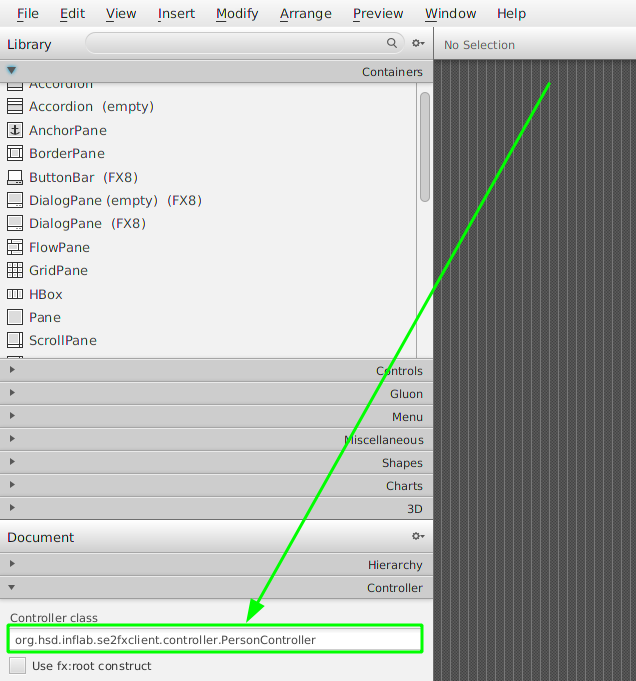
\includegraphics[width=\linewidth]{images/eclipse26_set_controller_in_fxml.png}
    \caption{Set controller in view}
    \label{fig:setcontrollerinview}
\end{figure}


\newpage
\subsubsection{View erstellen}
\label{sec:createview}
Aus der \textit{Containers} Sektion im linken
Panel den Container \textit{ButtonBar} in den BOTTON Bereich
der BorderPane ziehen:
\begin{figure}[!ht]
    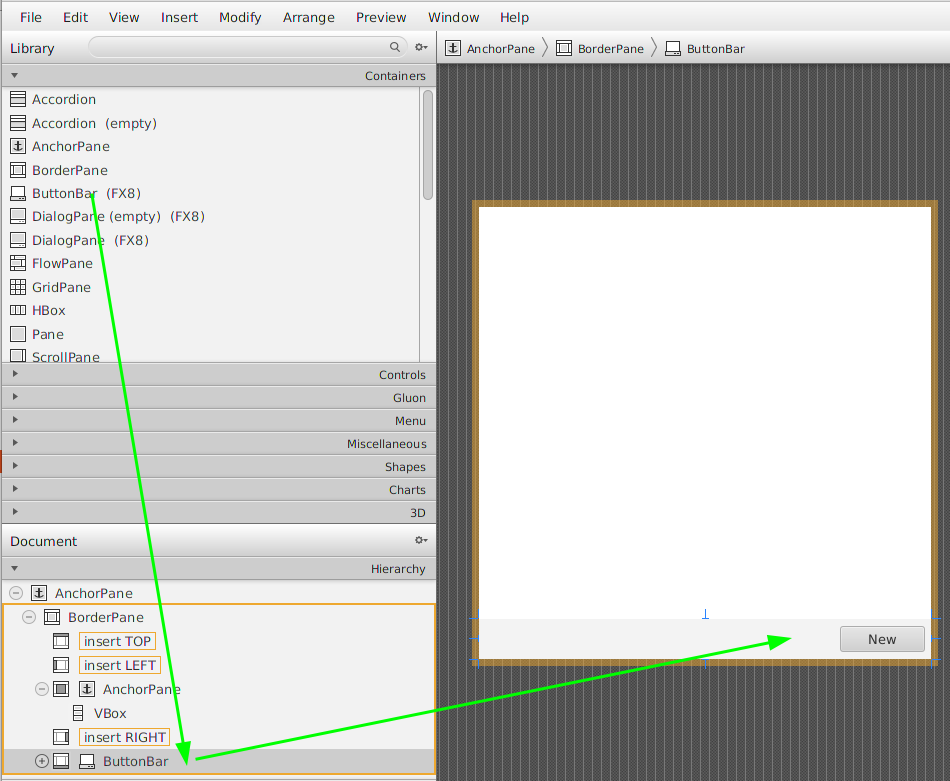
\includegraphics[width=\linewidth]{images/eclipse27_insert_buttonbar.png}
    \caption{Insert ButtonBar}
    \label{fig:insertbuttonbar}
\end{figure}

\newpage
den Button doppelklicken und in \textit{New} umbennen:
\begin{figure}[!ht]
    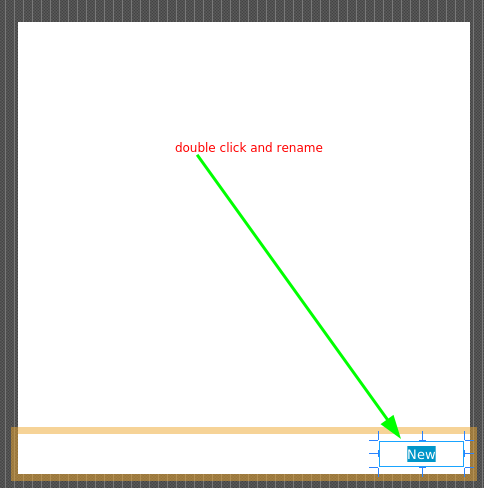
\includegraphics[width=\linewidth]{images/eclipse28_rename_button.png}
    \caption{Rename Button}
    \label{fig:renamebutton}
\end{figure}

\newpage
den Button anklicken, die Sektion \textit{Code} im rechten Panel anwählen
und dort die Methode \textit{addNewPerson} einfügen:
\begin{figure}[!ht]
    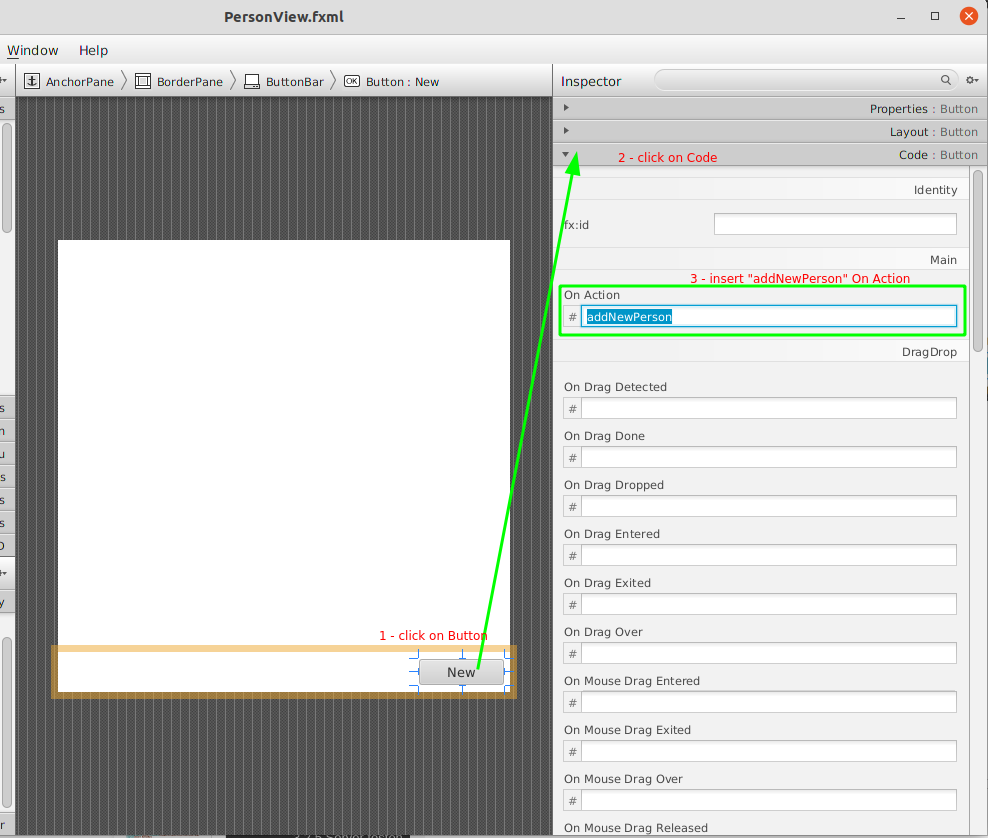
\includegraphics[width=\linewidth]{images/eclipse29_connect_method.png}
    \caption{Connect button to method}
    \label{fig:connectbuttontomethod}
\end{figure}

\newpage
aus der Sektion \textit{Containers} im linken Panel den Container \textit{AnchorPane}
in die mittlere Zelle der \textit{BorderPane} ziehen:
\begin{figure}[!ht]
    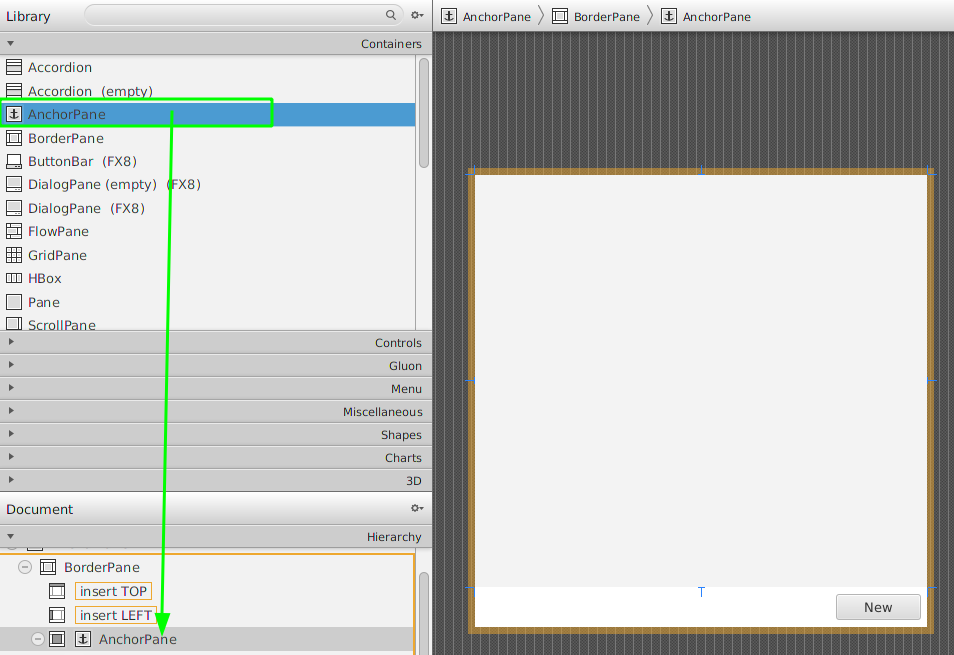
\includegraphics[width=\linewidth]{images/eclipse30_insert_anchorpane.png}
    \caption{Insert AnchroPane}
    \label{fig:insertanchorpane}
\end{figure}

\newpage
aus der Sektion \textit{Containers} im linken Panel den Container \textit{VBox}
in die \textit{AnchorPane} ziehen, und im rechten Panel unter der Sektion
\textit{Layout} das Layout anpassen (so wie man es schön findet...):
\begin{figure}[!ht]
    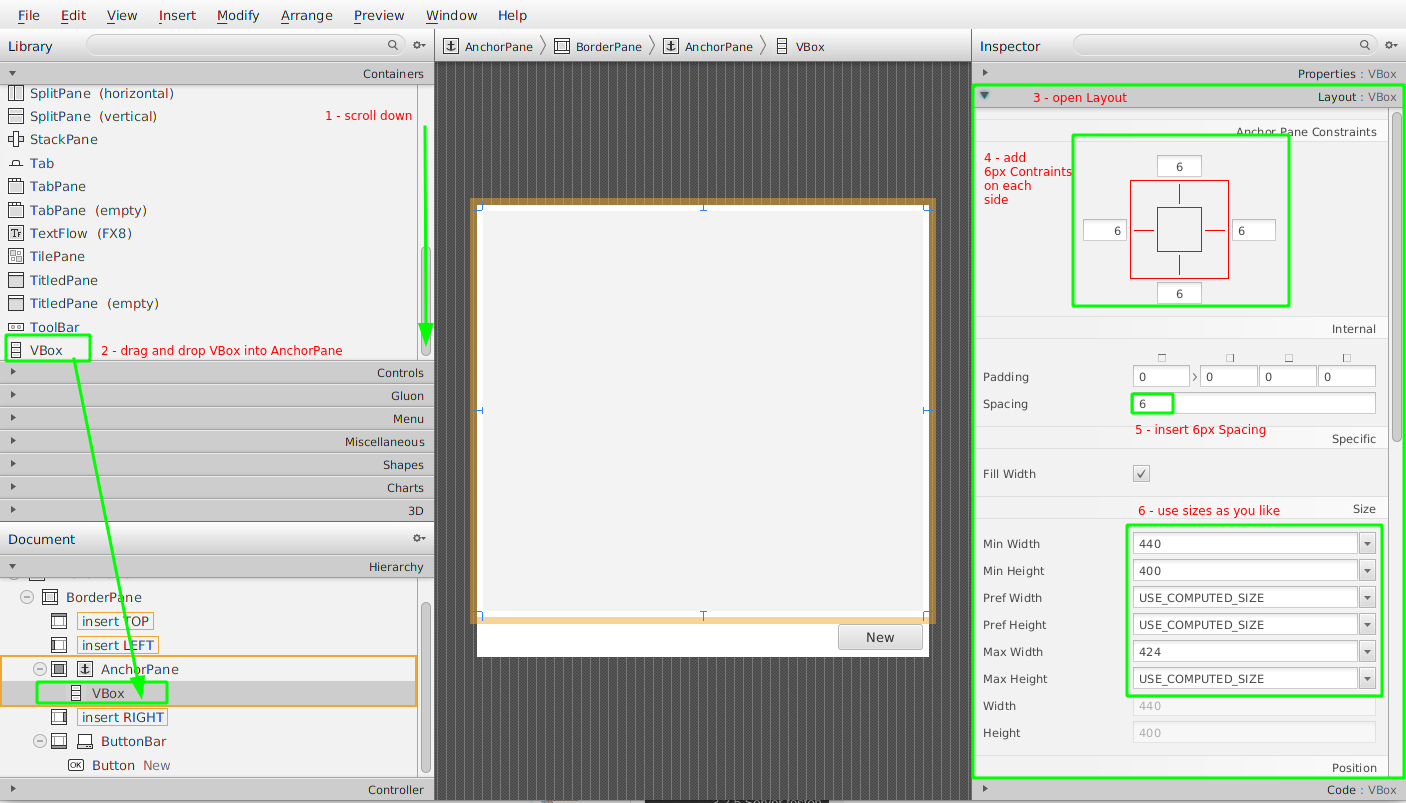
\includegraphics[width=\linewidth]{images/eclipse30_insert_vbox.png}
    \caption{Insert VBOx}
    \label{fig:insertvbox}
\end{figure}

\newpage
in der Sektion \textit{Code} im rechten Panel \textit{personsVBox} als \textit{fx:id}
eingeben und nicht vergessen das Dokument zu SPEICHERN!:
\begin{figure}[!ht]
    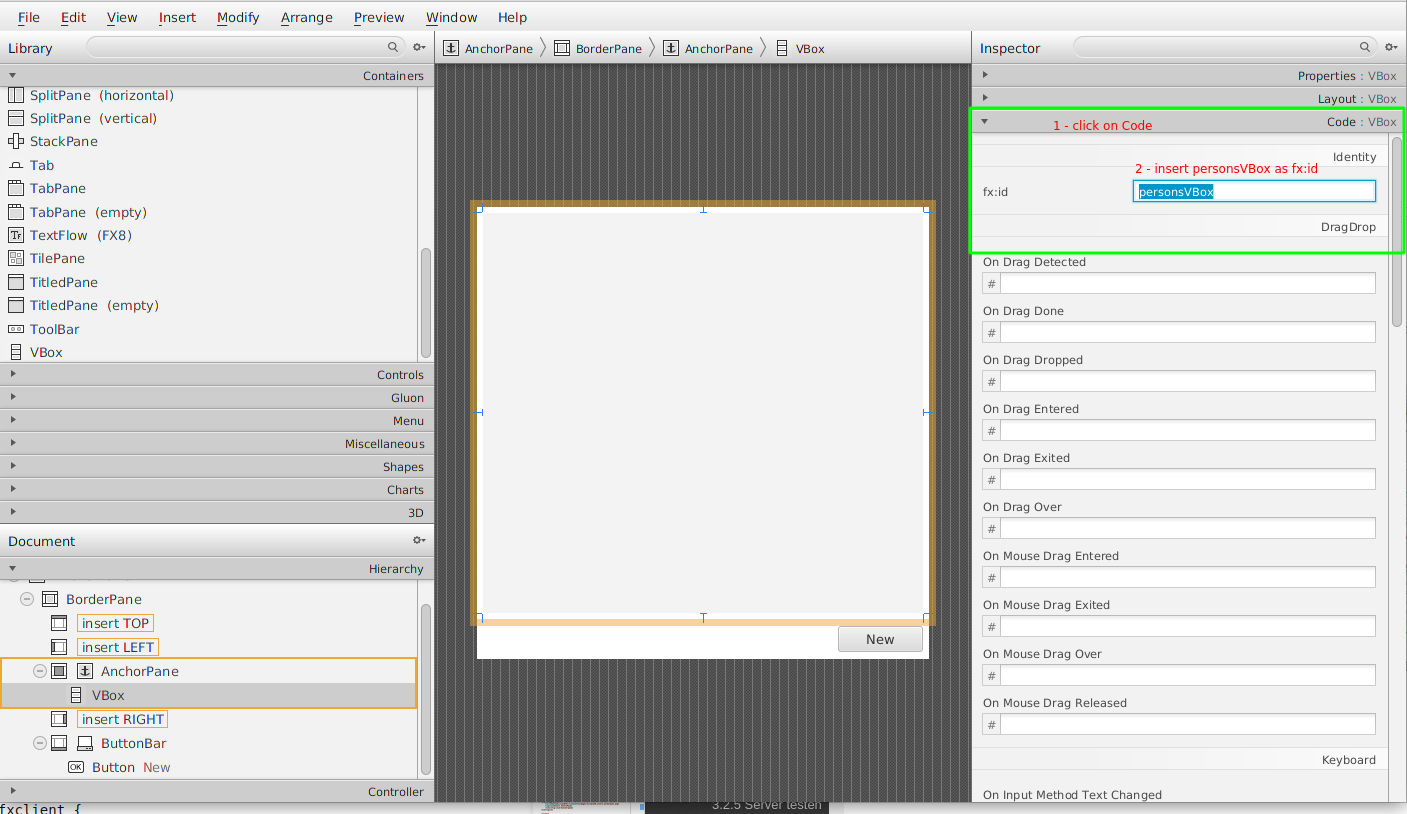
\includegraphics[width=\linewidth]{images/eclipse31_insert_id.png}
    \caption{Insert VBOx fx:id}
    \label{fig:insertvboxfxid}
\end{figure}

\newpage
\subsubsection{Finale Version von module-info.java}
\label{sec:finalizemoduleinfo}

Aufgrund der Tatsache dass ab Java9 JavaFX nicht mehr Teil des JDKs ist
sondern als Modul nachgeladen werden muss, haben wir die Datei module-info.java 
befüllt. Da das Modul nun die zusätzlichen Bibliotheken für HTTP und JSON benötigt,
müssen wir diese ebenfalls als required angeben. Zusätzlich fügen wir noch 
das Schlüsselwort transitive hinzu, um die entsprechenden Warnungen zu beseitigen.
Die finale Version von module-info.java sollte also wie folgt aussehen:

\begin{lstlisting}[language=java]
module org.hsd.inflab.se2fxclient {
    requires transitive javafx.controls;
    requires javafx.fxml;
    requires transitive javafx.graphics;
    requires org.apache.httpcomponents.httpcore;
    requires org.apache.httpcomponents.httpclient;
    requires org.json;

    opens org.hsd.inflab.se2fxclient.view to javafx.fxml;
    opens org.hsd.inflab.se2fxclient.controller to javafx.fxml;
    exports org.hsd.inflab.se2fxclient.controller;
    exports org.hsd.inflab.se2fxclient.view;
    exports org.hsd.inflab.se2fxclient.model;
}
\end{lstlisting}

\section{Full-Stack test}
\label{sec:fullstacktest}
\begin{enumerate}
    \item XAMPP oder XAMPP Docker starten
    \item Den Server aus \textit{Application.java} starten
    \item Den Client in \textit{App.java} starten
    \item Person anlegen mit \textit{New}
    \item Person umbennen im Textfeld und mit \textit{OK} bestätigen
    \item Person löschen mit \textit{Delete}
\end{enumerate}

\begin{figure}[!ht]
    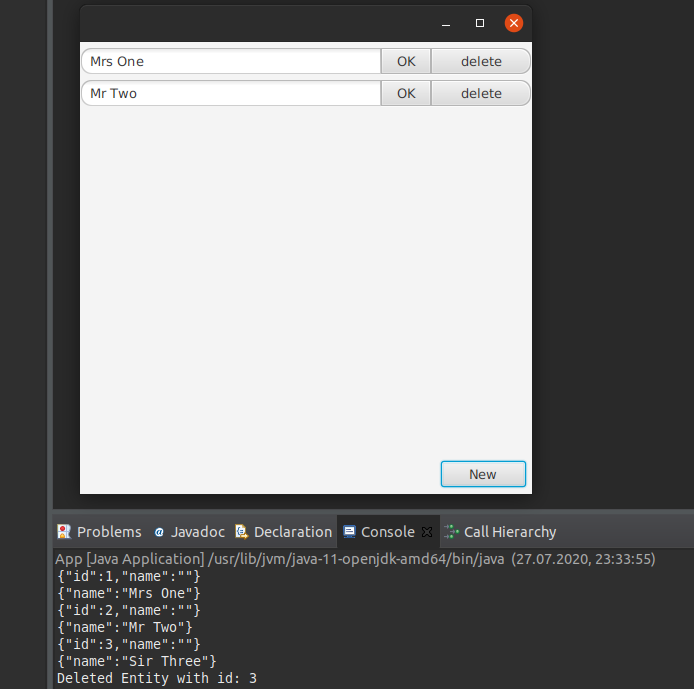
\includegraphics[width=\linewidth]{images/eclipse32_final_test.png}
    \caption{Final Test}
    \label{fig:finaltest}
\end{figure}

\end{document}